\documentclass[10pt,a4paper]{article}
\usepackage[utf8]{inputenc}
\usepackage[french]{babel}
\usepackage[T1]{fontenc}
\usepackage{amsmath}
\usepackage{amsfonts}
\usepackage{amssymb}
\usepackage{makeidx}
\usepackage{xcolor} 
\usepackage{graphicx}
\usepackage{lmodern}
\usepackage[many]{tcolorbox}
\usetikzlibrary{shadows}
\usepackage{kpfonts}
\usepackage{geometry}
\usepackage{xcolor} 
\usepackage{fancybox}
\usepackage{graphicx}
\usepackage{lmodern}
\author{KOUTEMA Ditoma}

\begin{document}
\newtcolorbox{shadedbox}{
  drop shadow southeast,
  breakable,
  enhanced jigsaw,
  colback=white,
}

\begin{shadedbox}
\begin{center}
\huge \textcolor{blue}{TP02 Python Django – Modèles et base de données}
\end{center}
\end{shadedbox}
%fin box%
\large{\begin{center}
fait par : 
\end{center}}
\begin{center}
\huge{KOUTEMA Ditoma}
\end{center}
\newpage
\tableofcontents
\newpage

\section{Mise en route}
\begin{enumerate}
\item 
\begin{itemize}
\item[]
\item La commande pour activer l'environnement virtuel :\\ \textcolor{blue}{source projetnotes/bin/activate}
\item Version de python : \textcolor{blue}{Python 3.10.12}
\item Version de django : \textcolor{blue}{4.2.6}
\end{itemize}

\item 
\begin{itemize}
\item[]
\item Arborescence de mon projet : \\\\
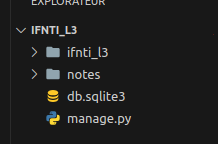
\includegraphics[scale=0.8]{1.png}
\item L'application \textbf{Notes} se trouve a la racine du projet IFNTI\_L3\\
\item L'application notes n'est pas dans le dossier ifnti\_l3 parce que, le dossier ifnti\_l3 est le dossier de configuration de toutes applications crées dans le projet.\\
\item Si l'application notes s'y trouvait alors, l'application notes ne va pas fonctionné tout simplement.
\end{itemize}
\end{enumerate}

\section{Configuration de la base de données}

\begin{enumerate}
\item 
\begin{itemize}
\item[]
\item Le moteur de base de donnée utilisé par défaut est  : \textcolor{blue}{sqlite3}

\item Les caractéristiques des bases de donnée de ce type la sont : \\
\begin{itemize}
\item[•] C'est un système de gestion de base de données relationnelle (SGBDR) open source.
\item[•] Il est très rapide.
\item[•] Il est multi-plateformes
\item[•] Il prend en charge les bases de données qui peuvent être très grandes; Actuellement, la limite est de 2 To
\item[•] On peut le stocker dans les fichiers.
\end{itemize}
\item Je ne pourrai pas l'utiliser en production car il a une limite de stockage.
\end{itemize}
\item Valeur du Time-Zone de lomé est : \textcolor{blue}{TIME\_ZONE = 'UTC'}




\item 
\begin{itemize}
\item[]
\item Le type de \textbf{INSTALLED\_APPS}  est une \textcolor{blue}{: list}.
\item Cette constante contient actuellement toutes les applications crées pendant la création du projet.
\end{itemize}

\item 
\begin{itemize}
\item[]
\item La commande pour lancer un serveur : \textcolor{blue}{py manage.py runserver}.
\item Cette constante contient actuellement toutes les applications crées pendant la création du projet.
\item Le texte en \textcolor{red}{rouge} signifie que les migrations ne sont pas encore exécutées pour l'application ifnti\_l3.
\item Pour régler le problème il suffit de lancer la commande donnée juste dans le texte en rouge : \textcolor{blue}{py manage.py migrate}
\end{itemize}
\end{enumerate}

\section{Création des modèles}
\begin{enumerate}
\item[] Un modèle est la source unique et définitive d’informations sur nos données.

\item Le fichier models.py contient une importation et un commentaire.\\
Ce code veut dire qu'on import les models issus de la classe django.db.


\item Code : 
\begin{verbatim}
from django.db import models

# Create your models here.
class Personne(models.Model):
    nom = models.CharField(max_length=50)
    prenom = models.CharField(max_length=50)
    sexe = models.TextChoices = [("M", "Masculin"),("F", "Femini"),]
    date_naissance = models.DateField()

    class Meta:
        asbtract = True


class Niveau(models.Model):
    nom = models.CharField(max_length=2, unique=True)
    pass


class Enseignant(Personne):
    pass


class Matiere(models.Model):
    nom = models.CharField(max_length=50, unique=True)
    enseignant = models.ForeignKey(Enseignant, on_delete=models.CASCADE)
    niveau = models.ForeignKey(Niveau, on_delete=models.CASCADE)
    


class Eleve(Personne):
    id=models.BigAutoField(primary_key=True)
    nom = models.CharField(max_length=30)
    niveau = models.ForeignKey(Niveau, on_delete=models.CASCADE)
    matiere = models.ManyToManyField(Matiere)



class Note(models.Model):
    eleve = models.ForeignKey(Eleve, on_delete=models.CASCADE)
    valeur = models.FloatField(max_length=30, null=True)
\end{verbatim}
\end{enumerate}

\section{Activation des modèles}

\begin{enumerate}
\item
\begin{itemize}
\item[]
\item[•] Contenu de INSTALL\_APPS : \\
\begin{verbatim}
INSTALLED_APPS = [
    'django.contrib.admin',
    'django.contrib.auth',
    'django.contrib.contenttypes',
    'django.contrib.sessions',
    'django.contrib.messages',
    'django.contrib.staticfiles',
    'notes.apps.NotesConfig',
]
\end{verbatim}
\item[•] NotesConfig est une classe qui hérite de AppConfig qui contient le nom de l'application.
%\item[•] Le fichier \textcolor{blue}{NotesConfig} est une classe permettant la configuration de notre base de donnée. 
\item[•] Cette classe se trouve dans le fichier \textcolor{blue}{apps}
\end{itemize}

\item
\begin{itemize}
\item[]
\item[•] La commande pour lancer les migrations :\\ \textcolor{blue}{py manage.py makemigrations}\\
Cette commande permet de construire les migrations.\\\\
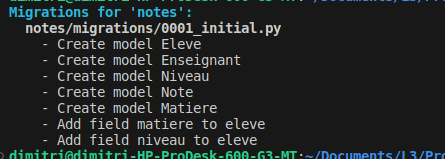
\includegraphics[scale=0.8]{2.png}\\\\
Sur le terminal je vois que les models : Eleve, Enseignant, Niveau, Note, Matiere, et les rélations établient entre matiere et eleve; niveau et eleve
\end{itemize}

\item
\begin{itemize}
\item[]
\item[•] Résultat de la commande : \textcolor{blue}{py manage.py sqlmigrate notes 0001}
\item[•] Il s'agit des requettes sql en dure.
\end{itemize}

\item
\begin{itemize}
\item[]
\item[•] Commande que j'ai lancée : \textcolor{blue}{py manage.py migrate}\\
\item[•] Le texte qui s'affiche en \textbf{rouge} demande de relancer la migration.



\end{itemize}

\end{enumerate}

















\end{document}